%% 
%% Copyright 2007-2025 Elsevier Ltd
%% 
%% This file is part of the 'Elsarticle Bundle'.
%% ---------------------------------------------
%% 
%% It may be distributed under the conditions of the LaTeX Project Public
%% License, either version 1.3 of this license or (at your option) any
%% later version.  The latest version of this license is in
%%    http://www.latex-project.org/lppl.txt
%% and version 1.3 or later is part of all distributions of LaTeX
%% version 1999/12/01 or later.
%% 
%% The list of all files belonging to the 'Elsarticle Bundle' is
%% given in the file `manifest.txt'.
%% 
%% Template article for Elsevier's document class `elsarticle'
%% with harvard style bibliographic references

\documentclass[preprint,12pt,authoryear]{elsarticle}

%% Use the option review to obtain double line spacing
%% \documentclass[authoryear,preprint,review,12pt]{elsarticle}

%% Use the options 1p,twocolumn; 3p; 3p,twocolumn; 5p; or 5p,twocolumn
%% for a journal layout:
%% \documentclass[final,1p,times,authoryear]{elsarticle}
%% \documentclass[final,1p,times,twocolumn,authoryear]{elsarticle}
%% \documentclass[final,3p,times,authoryear]{elsarticle}
%% \documentclass[final,3p,times,twocolumn,authoryear]{elsarticle}
%% \documentclass[final,5p,times,authoryear]{elsarticle}
%% \documentclass[final,5p,times,twocolumn,authoryear]{elsarticle}

%% For including figures, graphicx.sty has been loaded in
%% elsarticle.cls. If you prefer to use the old commands
%% please give \usepackage{epsfig}

%% The amssymb package provides various useful mathematical symbols
\usepackage{amssymb}
%% The amsmath package provides various useful equation environments.
\usepackage{amsmath}
\DeclareMathOperator*{\argmin}{arg\,min}
%% The amsthm package provides extended theorem environments
%% \usepackage{amsthm}
\usepackage{xcolor}
%% The lineno packages adds line numbers. Start line numbering with
%% \begin{linenumbers}, end it with \end{linenumbers}. Or switch it on
%% for the whole article with \linenumbers.
%% \usepackage{lineno}
\usepackage{url}
\usepackage{xurl}  % Allow URL breaks at any character
\usepackage{booktabs}
\usepackage{multirow}
\usepackage{tikz}
\usetikzlibrary{shapes.geometric, arrows.meta, positioning, patterns, decorations.pathmorphing, calc}
\usepackage{graphicx}
\usepackage{subcaption}

% Custom algorithm environment (no external packages required)
\newcounter{alg}
\renewcommand{\thealg}{\arabic{alg}}
\makeatletter
\newenvironment{algorithm}[1][t]{%
  \refstepcounter{alg}%
  \def\@captype{figure}%
  \begin{minipage}{\linewidth}%
  \hrule\vspace{4pt}%
  \textbf{Algorithm \thealg.} %
}{%
  \vspace{4pt}\hrule%
  \end{minipage}%
  \vspace{8pt}%
}
\makeatother
% Algorithmic commands
\newenvironment{algorithmic}[1][]{\begin{list}{}{\setlength{\leftmargin}{1.5em}\setlength{\itemsep}{1pt}\setlength{\parsep}{0pt}}\small}{\end{list}}
\newcommand{\REQUIRE}{\item[\textbf{Input:}]}
\newcommand{\ENSURE}{\item[\textbf{Output:}]}
\newcommand{\STATE}{\item}
\newcommand{\FOR}[1]{\item \textbf{for} #1 \textbf{do}}
\newcommand{\ENDFOR}{\item \textbf{end for}}
\newcommand{\IF}[1]{\item \textbf{if} #1 \textbf{then}}
\newcommand{\ENDIF}{\item \textbf{end if}}
\newcommand{\RETURN}{\item \textbf{return} }
\newcommand{\COMMENT}[1]{\hfill \textit{// #1}}
\newcommand{\AND}{\textbf{ and }}

\journal{Waste Management}

\begin{document}

\begin{frontmatter}

%% Title, authors and addresses

%% use the tnoteref command within \title for footnotes;
%% use the tnotetext command for theassociated footnote;
%% use the fnref command within \author or \affiliation for footnotes;
%% use the fntext command for theassociated footnote;
%% use the corref command within \author for corresponding author footnotes;
%% use the cortext command for theassociated footnote;
%% use the ead command for the email address,
%% and the form \ead[url] for the home page:
%% \title{Title\tnoteref{label1}}
%% \tnotetext[label1]{}
%% \author{Name\corref{cor1}\fnref{label2}}
%% \ead{email address}
%% \ead[url]{home page}
%% \fntext[label2]{}
%% \cortext[cor1]{}
%% \affiliation{organization={},
%%            addressline={}, 
%%            city={},
%%            postcode={}, 
%%            state={},
%%            country={}}
%% \fntext[label3]{}

\title{Solid Waste Classification Using Computer Vision Techniques} %% Article title

%% use optional labels to link authors explicitly to addresses:
%% \author[label1,label2]{}
%% \affiliation[label1]{organization={},
%%             addressline={},
%%             city={},
%%             postcode={},
%%             state={},
%%             country={}}
%%
%% \affiliation[label2]{organization={},
%%             addressline={},
%%             city={},
%%             postcode={},
%%             state={},
%%             country={}}

\author{Burak Akdemir, Sinan Topçakar, Eren Korkmaz, Prof. Dr. Seniha Esen Yüksel Erdem} %% Author name

%% Author affiliation
\affiliation{organization={Hacettepe University},%Department and Organization
            addressline={Üniversiteler, Hacettepe Beytepe Kampüsü 25 A}, 
            city={Ankara},
            postcode={06800}, 
            state={Çankaya},
            country={Turkey}}

%% Abstract
\begin{abstract}
Automated waste classification on high-throughput conveyor systems requires material discrimination beyond visual appearance. We present a framework combining RGB and thermal imaging for classifying municipal solid waste into four categories: metal, plastic, glass, and paper. The system introduces an active heating zone where objects acquire material-specific thermal signatures as they travel along the conveyor, while independently operating RGB and thermal cameras record their trajectories. Since the cameras lack hardware synchronization and timestamps are unreliable, we develop a feature-based spatial-temporal registration method that achieves 2.27-pixel spatial alignment and 4.68-pixel mean temporal registration error across 281,439 validated frame pairs, enabling thermal time-series extraction from 550 tracked object trajectories.

Leveraging these registered sequences, we systematically evaluate eight classification methods on thermal intensity time-series. SVM with five statistical features achieves F1 = 0.678, comparable to deep learning approaches (BiGRU F1 = 0.676, InceptionTime F1 = 0.672), while all sequence-based methods substantially outperform the peak histogram baseline of \citet{GUNDUPALLI201713} (F1 = 0.550), confirming that temporal shape encodes material-discriminative information beyond peak statistics. Glass is most reliably classified (F1 = 0.786) owing to its distinctively low thermal response, while metal presents the greatest challenge (F1 = 0.490) due to high thermal variability.

We release ThermalRGBTrash, an RGB-thermal video dataset for conveyor-based waste classification, comprising 550 tracked object trajectories across four material classes with synchronized thermal time-series capturing dynamic heating and cooling responses unavailable in static imagery.
\end{abstract}

%%Graphical abstract
\begin{graphicalabstract}
%\includegraphics{grabs}
\end{graphicalabstract}

%%Research highlights
\begin{highlights}
\item SVM with five thermal features achieves F1 = 0.678, matching deep learning approaches (BiGRU F1 = 0.676, InceptionTime F1 = 0.672)
\item All sequence-based classifiers outperform peak histogram features (Gundupalli F1 = 0.550), confirming temporal shape encodes material information
\item Feature-based registration achieves 2.27-pixel spatial and 4.68-pixel temporal alignment across 281,439 frame pairs without hardware synchronization
\item Release of ThermalRGBTrash, an RGB-thermal dataset for conveyor-based waste classification (550 tracked object trajectories)
\end{highlights}

%% Keywords
\begin{keyword}
waste classification \sep thermal imaging \sep deep learning \sep conveyor system \sep time-series classification
\end{keyword}

\end{frontmatter}

%% Add \usepackage{lineno} before \begin{document} and uncomment 
%% following line to enable line numbers
%% \linenumbers

%% main text
%%

%% Use \section commands to start a section
\section{Introduction}\label{sec:intro}

The rapid increase in municipal solid waste (MSW), driven by population growth and consumerism, presents a significant environmental challenge \citep{minelgaite2019}. Manual sorting of MSW remains the most common approach, but it suffers from limited throughput, health risks for workers, and inconsistent sorting decisions caused by fatigue \citep{Ferro2024, Gundupalli2017, ErgonomicAssessment, Giel2025}. Computer vision systems offer an alternative that can operate continuously without exposing humans to hazardous conditions \citep{LuChen2022}.

Deep learning models have shown promising results for waste detection and classification. Detection architectures based on YOLO variants achieve real-time performance: \citet{ma2024dsyolo} developed DSYOLO-Trash by integrating Convolutional Block Attention Module (CBAM) and Contextual Transformer Networks (CotNet) into YOLOv5, combined with DeepSORT tracking for continuous waste monitoring. \citet{chen2024mrsyolo} proposed MRS-YOLO, incorporating SlideLoss-IoU for small object detection and RepViT Transformer modules for enhanced feature extraction, achieving 3.6\% mAP improvement over YOLOv8. \citet{yolov12waste2025} applied YOLOv12 with REST Effective Layer Aggregation Network (REST-ELAN) for conveyor-based detection, reaching 78\% mAP across six waste categories. For classification, \citet{nahiduzzaman2025tricascade} proposed a three-stage hierarchical framework using parallel lightweight depth-wise separable CNNs with Ensemble Extreme Learning Machines (En-ELM), progressing from binary biodegradable/non\-biodegradable classification to 36-class fine-grained categorization. \citet{kashaf2024vitwm} demonstrated that Vision Transformers combined with CNN and RNN feature extractors achieve 98.17\% accuracy through transfer learning on combined TrashNet and Kaggle datasets. However, these high accuracies (96--99\%) were achieved on curated benchmark datasets such as TrashNet~\citep{thung2016trashnet}, TACO~\citep{proenca2020taco}, and ZeroWaste~\citep{bashkirova2022zerowaste} with controlled lighting, isolated objects, and clean backgrounds, which are conditions rarely present in industrial Material Recovery Facilities. Moreover, all these systems rely exclusively on RGB cameras operating in the visible spectrum (0.4--0.7 $\mu$m), which cannot differentiate materials with similar visual appearance but distinct material composition. For example, clear glass and clear plastic appear nearly identical visually but require completely different recycling processes \citep{LuChen2022}.

Alternative sensing modalities can provide material discrimination unavailable from RGB. Hyperspectral imaging systems for waste sorting require capital investment of \$100,000--500,000 for SWIR-range cameras with calibrated illumination and specialized classification software~\citep{surfaceoptics2025}. X-ray transmission (XRT) sorters cost \$200,000--800,000 and require radiation shielding infrastructure, safety compliance, and specialized operators~\citep{konstantinidis2023systematic}. Thermal cameras operating in the LWIR band (7.5--14~$\mu$m) offer a more accessible alternative at \$5,000--20,000, functioning under ambient lighting conditions without controlled environments~\citep{GUNDUPALLI201713}.

Thermal imaging in the LWIR band (7.5--14 $\mu$m) captures material-specific behaviors related to thermal conductivity, specific heat capacity, and emissivity \citep{GUNDUPALLI201713}. \citet{GUNDUPALLI201713} pioneered thermal imaging for waste classification using an enclosed hot chamber with controlled heating, extracting emissivity-based features to achieve 85--96\% accuracy across four material types (glass, metal, plastic, paper). Subsequent work by the same group extended this approach to e-waste separation using similar static thermal imaging protocols \citep{10.1115/DETC2016-59842, 10.1115/1.4047485}. \citet{kumar2020thermal} proposed an electrical analogy method that models heat conduction as an RC ladder network, estimating thermal diffusivity and conductivity from the thermal delay $\tau_{TD}$, defined as the time for a material to reach 63\% of applied temperature. However, these approaches require enclosed hot chambers with 30--60 second dwell times per object, limiting practical throughput. No previous work has demonstrated thermal classification from objects moving continuously through open heating zones at conveyor speeds, which would enable real-time industrial deployment without the throughput constraints of enclosed chambers.

Combining RGB with complementary sensing modalities can address the limitations of each individual sensor. \citet{ji2023rgbnir} fused RGB with near-infrared (NIR) spectral features to classify plastic waste by material type and color, demonstrating improved discrimination over RGB-only approaches. \citet{li2022rgbd_cdw} proposed RGB-D fusion models combining color images with depth data from laser line-scanning for construction and demolition waste detection using Mask R-CNN. \citet{casao2024spectralwaste} introduced SpectralWaste, the first industrial RGB-hyperspectral dataset for waste sorting, demonstrating that multimodal fusion improves segmentation in cluttered recycling facility environments. For cross-modal image matching between RGB and thermal modalities, \citet{tuzcuoglu2024xoftr} proposed XoFTR, a Transformer-based feature matching method using masked image modeling pre-training to handle the significant texture and intensity differences between visible and thermal images. For waste classification with sequential data, hybrid CNN-LSTM architectures combining convolutional feature extraction with recurrent temporal modeling achieve 95.45\% accuracy on TrashNet~\citep{lilhore2024cnnlstm}, while Vision Transformers adapted for waste classification reach 96.98\% accuracy through transfer learning~\citep{srinilta2021vitwaste}. However, systematic evaluation of thermal time-series classification methods for waste sorting on continuous conveyor systems remains unexplored.

The critical gap in prior work is the absence of methods that exploit \emph{dynamic} thermal signatures, specifically the time-varying heating and cooling patterns that encode material-specific thermal properties, for waste classification on continuous conveyor systems. Prior thermal approaches rely on static measurements requiring enclosed chambers, while RGB-based methods cannot capture thermodynamic properties regardless of model sophistication.

To address this gap, we propose a framework combining RGB and thermal imaging for solid waste classification, with systematic evaluation of thermal time-series classification methods. The main contributions are:

\begin{enumerate}
    \item We design an open-air heating zone that exposes material-specific thermal signatures as objects pass continuously, avoiding the throughput limitations of enclosed chambers.

    \item We develop a spatial-temporal registration method for unsynchronized RGB-thermal cameras, combining learned feature matching (SuperPoint-SuperGlue) with adaptive temporal search to achieve 2.27-pixel spatial and 4.68-pixel temporal alignment without hardware synchronization or reliable timestamps.

    \item We systematically benchmark eight thermal classification methods---including SVM, recurrent networks (BiLSTM, BiGRU), convolutional architectures (TCN, 1D~CNN, InceptionTime), Transformer, and MiniRocket---on thermal intensity time-series extracted from 550 tracked object trajectories. SVM with five statistical features (F1 = 0.678) achieves competitive performance with deep learning approaches, while all sequence-based methods outperform the peak histogram baseline (F1 = 0.550), confirming that temporal dynamics encode material-discriminative information.

    \item We release ThermalRGBTrash, the first dataset containing registered RGB-thermal video pairs with thermal signatures for conveyor-based waste classification research, comprising 550 tracked trajectories across four material classes.
\end{enumerate}

\section{System Overview}\label{sec:system_overview}
In Figure \ref{fig:technical_drawing_of_conveyor.png}, the proposed system consisting of three major parts (conveyor module, heating module, and data acquisition module) is shown. The conveyor module consists of a conveyor belt (160 cm $\times$ 40 cm) operating at 1.8 cm/s. The heating module includes a 2500 Watt electric heater positioned 60 cm above the conveyor belt. The heater is directed towards the conveyor and surrounded by isolators that concentrate heat on a specific area, which is called the heating zone. Objects moving on the conveyor undergo two sequential stages: first, an active heating stage where objects pass through the heating zone, followed by a passive cooling stage at ambient conditions. Observing an object undergoing these stages reveals its thermal characteristics. For data acquisition, a thermal camera (FLIR T420, 320 $\times$ 240 resolution) and an RGB camera (1280 $\times$ 720 resolution) are used in tandem at 30 FPS, with spatial correspondence established via homography transformation. The experimental setup represents a controlled laboratory environment designed to isolate thermal material signatures; key differences from industrial Material Recovery Facilities include single-object scenes, controlled ambient lighting, and lower throughput.

Videos obtained from the cameras are aligned in both spatial and temporal domains. The spatial alignment results in a homography matrix (H) that encapsulates the geometric transformation from the RGB image to the thermal image. In the temporal domain, alignment involves establishing a frame-to-frame mapping between the thermal and RGB video frames. This frame-to-frame correspondence is necessary to overcome two challenges in the proposed setup: the difficulty in simultaneously initiating capture on both cameras and the unreliability of embedded frame timestamps, which prevent their use for direct frame matching. The 16$\times$ resolution difference between the cameras affects the registration pipeline: RGB frames are warped to thermal resolution, preserving thermal pixel fidelity at the cost of RGB spatial detail.

Once spatial and temporal alignments are established, the next step is instance segmentation: to find the contours of MSW moving on the conveyor, frames of the RGB video are segmented. RGB images are used for segmentation due to the higher spatial resolution of the RGB camera and the extensive availability of segmentation models pre-trained on RGB datasets. The masks obtained, which identify the contours of MSW, on RGB images are mapped onto thermal images using H so that the average pixel intensity for each MSW can be tracked while moving on the conveyor. Tracking the average of pixel values within a mask as the MSW move on the conveyor results in an array of values which indicates the temperature change of the MSW. The temperature change of MSW as they move on the conveyor is treated as a time series which is used for classification of the object according to material type. The complete computational pipeline is illustrated in Figure~\ref{fig:pipeline}. In addition to thermal intensity time-series, the pipeline extracts per-frame class probability distributions from the RGB segmentation model, enabling analysis of RGB-based classification performance alongside thermal-based approaches.

\begin{figure}[t]
    \centering
    \includegraphics[width=\textwidth]{images/technical_drawing_of_conveyor.png}
    \caption{Technical drawing of the proposed system. Objects are placed on the conveyor from the right side and move leftward, first passing through the active heating zone and then the passive cooling zone where their distinct thermal characteristics are exposed.}
    \label{fig:technical_drawing_of_conveyor.png}
\end{figure}

\begin{figure}[t]
    \centering
        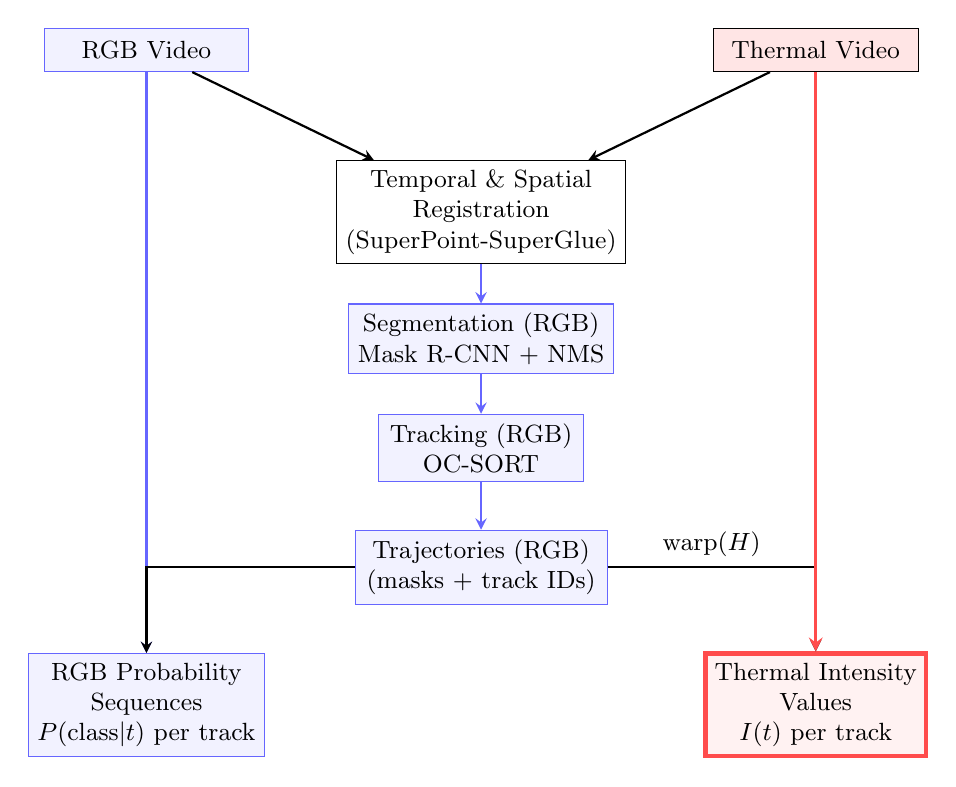
\begin{tikzpicture}[
            node distance=0.6cm,
            box/.style={rectangle, draw, minimum width=2.6cm, minimum height=0.55cm,
                        align=center, font=\small},
            rgbbox/.style={rectangle, draw=blue!60, fill=blue!5, minimum width=2.6cm,
                          minimum height=0.55cm, align=center, font=\small},
            emphbox/.style={rectangle, draw=red!70, line width=1.5pt, fill=red!5,
                           minimum width=2.6cm, minimum height=0.55cm,
                           align=center, font=\small\bfseries},
            arrow/.style={->, >=stealth, thick},
            redarrow/.style={->, >=stealth, thick, red!70, line width=1.2pt},
            scale=0.85
        ]

        % ===== INPUT LAYER =====
        \node[rgbbox] (rgb) at (-5,0) {RGB Video};
        \node[box, fill=red!10] (thermal) at (5,0) {Thermal Video};

        % ===== REGISTRATION (uses both) =====
        \node[box, below=1.4cm of $(rgb)!0.5!(thermal)$, minimum width=2.2cm] (reg) {Temporal \& Spatial\\Registration\\(SuperPoint-SuperGlue)};

        % ===== RGB-ONLY PROCESSING PATH =====
        \node[rgbbox, below=0.5cm of reg] (det) {Segmentation (RGB)\\Mask R-CNN + NMS};
        \node[rgbbox, below=0.5cm of det] (track) {Tracking (RGB)\\OC-SORT};

        % ===== TRACKING OUTPUT: Trajectories =====
        \node[rgbbox, below=0.6cm of track, minimum width=3.2cm] (traj) {Trajectories (RGB)\\(masks + track IDs)};

        % ===== SPLIT FROM TRAJECTORIES =====
        % Calculate y-position below traj, use x from rgb/thermal
        \path (traj.south) ++(0,-1.5) coordinate (below_traj);
        % Left: RGB probabilities (x-aligned with RGB Video)
        \node[rgbbox] at (-5,0 |- below_traj) (rgb_prob) {RGB Probability\\Sequences\\$P(\text{class}|t)$ per track};
        % Right: Thermal intensity values (x-aligned with Thermal Video)
        \node[emphbox, font=\small] at (5,0 |- below_traj) (thermal_ext) {Thermal Intensity\\Values\\$I(t)$ per track};

        % ===== ARROWS =====
        % Registration inputs (both videos feed into registration)
        \draw[arrow] (rgb) -- (reg);
        \draw[arrow] (thermal) -- (reg);

        % RGB video to RGB Probability Sequences (straight line)
        \draw[arrow, blue!60] (rgb) -- (rgb_prob);

        % RGB processing path
        \draw[arrow, blue!60] (reg) -- (det);
        \draw[arrow, blue!60] (det) -- (track);

        % Tracking to Trajectories
        \draw[arrow, blue!60] (track) -- (traj);

        % Trajectories split to RGB probabilities and Thermal Extraction
        \draw[arrow] (traj) -| (rgb_prob);
        \draw[arrow] (traj) -| (thermal_ext) node[pos=0.25, above, font=\small] {warp($H$)};

        % Thermal video to extraction (straight line)
        \draw[redarrow] (thermal) -- (thermal_ext);

        \end{tikzpicture}
    \caption{Computational pipeline for feature extraction. Segmentation and tracking operate on RGB frames only; the resulting trajectories enable extraction of per-track class probability sequences $P(\text{class}|t)$ and thermal intensity time-series $I(t)$ via homography transformation. The thermal output encodes material-specific thermal characteristics used for time-series classification.}
    \label{fig:pipeline}
\end{figure}

%% === RGB-THERMAL CONJUGATE FIGURE (Generated by thermal-visual-evidence-orchestrator) ===
\begin{figure}[t]
    \centering
    \begin{tabular}{@{}cc@{}}
        \includegraphics[width=0.48\textwidth]{images/exp_0852_eo_conjugate.png} &
        \includegraphics[width=0.48\textwidth]{images/exp_0852_th_conjugate.png} \\
        \small (a) Experiment 0852 RGB & \small (b) Experiment 0852 Thermal \\[6pt]
        \includegraphics[width=0.48\textwidth]{images/exp_0854_eo_conjugate.png} &
        \includegraphics[width=0.48\textwidth]{images/exp_0854_th_conjugate.png} \\
        \small (c) Experiment 0854 RGB & \small (d) Experiment 0854 Thermal
    \end{tabular}
    \caption{RGB-thermal conjugate pairs demonstrating modality complementarity. Glass appears darkest in thermal despite visual transparency; plastic exhibits highest thermal intensity; metal shows intermediate response.}
    \label{fig:visual_thermal_complementarity}
\end{figure}

The dual-modality approach exploits orthogonal information channels. RGB imaging captures surface appearance (color, texture, geometry) in the visible spectrum. Thermal imaging in the LWIR band (7.5--14~$\mu$m) measures radiance, which depends on surface emissivity and temperature; temporal changes reveal material-specific heating and cooling dynamics. These thermal behaviors differ across material classes~\citep{GUNDUPALLI201713}, providing discrimination unavailable from visual features alone. Figure~\ref{fig:visual_thermal_complementarity} demonstrates this complementarity: objects similar in the RGB domain can exhibit significant differences in the thermal domain.

\section{Materials and Methods}\label{Image Registration}

\subsection{Dataset}\label{subsec:dataset}

We release ThermalRGBTrash, a multimodal dataset for RGB-thermal waste classification on conveyor systems, combining spatially and temporally registered RGB-thermal video pairs with thermal time-series signatures for material classification. The dataset comprises two components: (1) 626 RGB frames with 3,953 instance-level COCO masks for segmentation training, and (2) 550 tracked object trajectories for time-series classification.

\begin{table}[h!]
    \centering
    \caption{ThermalRGBTrash dataset composition: segmentation instances (left) and classification trajectories (right).}\label{tab:dataset_combined}
    \begin{tabular}{lrr|lrrrr}
        \hline
        \multicolumn{3}{c|}{\textbf{Segmentation}} & \multicolumn{5}{c}{\textbf{Classification}} \\
        \textbf{Class} & \textbf{Count} & \textbf{\%} & \textbf{Split} & \textbf{Glass} & \textbf{Metal} & \textbf{Paper} & \textbf{Plastic} \\
        \hline
        Metal   & 2,277 & 57.6 & Train (60\%) & 79 & 79 & 59 & 113 \\
        Plastic & 771   & 19.5 & Val (20\%)   & 26 & 26 & 20 & 38 \\
        Paper   & 659   & 16.7 & Test (20\%)  & 27 & 26 & 19 & 38 \\
        Glass   & 246   & 6.2  & \textbf{Total} & \textbf{132} & \textbf{131} & \textbf{98} & \textbf{189} \\
        \hline
    \end{tabular}
\end{table}

Object trajectories are partitioned into stratified train/validation/test splits (60/20/20) with fixed random seed, ensuring proportional class representation across splits. Each trajectory comprises thermal intensity measurements capturing material-specific thermal signatures.

\subsection{Image Registration}\label{subsec:Img_reg}
RGB and thermal video streams must be registered in both spatial and temporal domains to enable accurate thermal signature extraction: spatial alignment ensures that segmentation masks obtained from RGB frames correctly delineate object boundaries in the thermal domain, while temporal alignment establishes frame-to-frame correspondences necessary for constructing per-track thermal time-series. Spatial registration establishes pixel correspondence between RGB and thermal frames; temporal registration identifies frame-to-frame matches between unsynchronized video streams. Both employ feature-based approaches: extract and match features, then select parameters minimizing the designed error metrics.

\begin{figure}[ht]
    \centering
    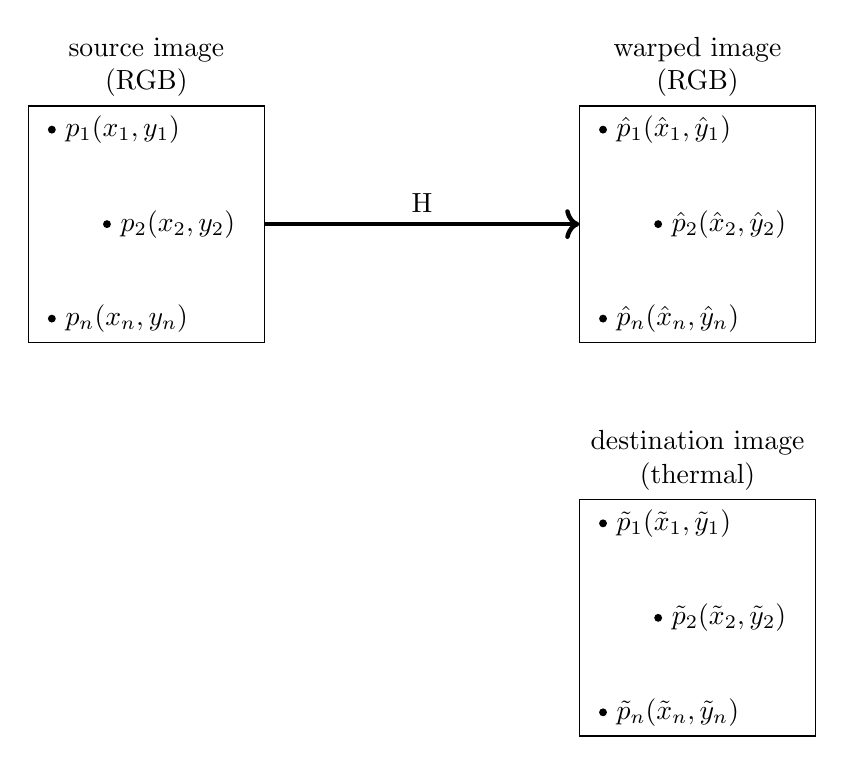
\begin{tikzpicture}
        % --- Source Image ---
        \node [above, align=center] at (1.5, 3) {source image \\ (RGB)};
        \draw[black] (0,0) rectangle (3,3);
        % Points in source image
        \fill[black] (0.3, 2.7) circle (0.05);
        \node[right] at (0.35, 2.7) {$p_1(x_1, y_1)$};
        \fill[black] (1.0, 1.5) circle (0.05);
        \node[right] at (1.05, 1.5) {$p_2(x_2, y_2)$};
        \fill[black] (0.3, 0.3) circle (0.05);
        \node[right] at (0.35, 0.3) {$p_n(x_n, y_n)$};

        % --- Warped Image ---
        \node [above, align=center] at (8.5, 3) {warped image \\ (RGB)};
        \draw[black] (7,0) rectangle (10,3);
        % Points in warped image
        \fill[black] (7.3, 2.7) circle (0.05);
        \node[right] at (7.35, 2.7) {$\hat{p}_1(\hat{x}_1, \hat{y}_1)$};
        \fill[black] (8.0, 1.5) circle (0.05);
        \node[right] at (8.05, 1.5) {$\hat{p}_2(\hat{x}_2, \hat{y}_2)$};
        \fill[black] (7.3, 0.3) circle (0.05);
        \node[right] at (7.35, 0.3) {$\hat{p}_n(\hat{x}_n, \hat{y}_n)$};

        % --- Destination Image ---
        \node [above, align=center] at (8.5, -2) {destination image \\ (thermal)};
        \draw[black] (7,-5) rectangle (10,-2);
        % Points in destination image
        \fill[black] (7.3, -2.3) circle (0.05);
        \node[right] at (7.35, -2.3) {$\tilde{p}_1(\tilde{x}_1, \tilde{y}_1)$};
        \fill[black] (8.0, -3.5) circle (0.05);
        \node[right] at (8.05, -3.5) {$\tilde{p}_2(\tilde{x}_2, \tilde{y}_2)$};
        \fill[black] (7.3, -4.7) circle (0.05);
        \node[right] at (7.35, -4.7) {$\tilde{p}_n(\tilde{x}_n, \tilde{y}_n)$};

        % --- Arrow with Homography Label ---
        \draw[ultra thick, ->] (3, 1.5) -- node[midway, above] {H} (7, 1.5);
    \end{tikzpicture}
    \caption{Coordinate systems for spatial registration. Feature points $p_i$ in the source RGB image are transformed via homography $H$ to warped coordinates $\hat{p}_i$. Registration accuracy is quantified by the displacement between warped positions and corresponding features $\tilde{p}_i$ detected in the thermal destination image.}
    \label{fig:images_to_be_aligned}
\end{figure}

Considering that the alignment process comprises both spatial and temporal components, a total alignment error metric that incorporates inaccuracies from both domains is formulated as:
\begin{equation}\label{eqn:total_RE}
    RE = RE_{\text{spatial}} + RE_{\text{temporal}}
\end{equation}
Details of spatial and temporal image registration are explained in Section~\ref{subsubsec:img_reg_spatial} and Section~\ref{subsubsec:img_reg_temporal} respectively.

\subsubsection{Image Registration in Spatial Domain}
\label{subsubsec:img_reg_spatial}

Spatial registration aligns the RGB source image with the thermal destination image through ROI extraction and homography estimation. ROI extraction uses HSV color segmentation (H$\in$[15,65], S$\in$[100,255], V$\in$[140,255]) targeting yellow fluorescent tape affixed to the conveyor frame, which delineates the ROI boundaries as illustrated in Figure~\ref{fig:roi_extraction}. Metal calibration markers with geometric patterns (T-junctions, crosses, corner brackets) are positioned within the field of view for cross-modal feature matching; metal's high thermal conductivity ensures rapid thermal equilibration, producing consistent edge gradients across modalities, while the geometric shapes provide canonical keypoint patterns (corners, junctions) that learned detectors reliably localize.

\begin{figure}[t]
    \centering
    \begin{subfigure}[b]{0.48\textwidth}
        \centering
        \includegraphics[width=\textwidth]{images/hsv_original_frame_900.png}
        \caption{Raw RGB frame}
        \label{fig:hsv_original}
    \end{subfigure}
    \hfill
    \begin{subfigure}[b]{0.48\textwidth}
        \centering
        \includegraphics[width=\textwidth]{images/hsv_mask_frame_900.png}
        \caption{HSV color mask}
        \label{fig:hsv_mask}
    \end{subfigure}

    \vspace{0.3cm}

    \begin{subfigure}[b]{0.48\textwidth}
        \centering
        \includegraphics[width=\textwidth]{images/hsv_bbox_frame_900.png}
        \caption{Detected bounding box}
        \label{fig:hsv_bbox}
    \end{subfigure}
    \hfill
    \begin{subfigure}[b]{0.48\textwidth}
        \centering
        \includegraphics[width=\textwidth]{images/hsv_cropped_frame_900.png}
        \caption{Extracted ROI}
        \label{fig:hsv_cropped}
    \end{subfigure}
    \caption{ROI extraction via HSV color segmentation. (a) Raw frame from RGB camera showing laboratory environment. (b) Binary mask from HSV thresholding detecting yellow fluorescent tape boundaries. (c) Bounding box computed from mask contours. (d) Cropped conveyor belt region with metal calibration markers for cross-modal feature matching.}
    \label{fig:roi_extraction}
\end{figure}

Handcrafted feature detectors achieve limited correspondence rates on cross-spectral imagery. On standard benchmarks, SIFT obtains only 21\% of estimates under 5-pixel error for thermal-visible pairs~\citep{thomas2025crossspectral}. We employ learned descriptors that have demonstrated superior cross-modal performance~\citep{tuzcuoglu2024xoftr,qin2023multispectral}: SuperPoint~\citep{detone2018superpoint} for keypoint detection (threshold = 0.0001) and SuperGlue~\citep{sarlin2020superglue} for correspondence matching (threshold = 0.2). Although trained on visible-spectrum imagery, these networks successfully match our metal calibration markers, whose corner and junction patterns match SuperPoint's training distribution (Synthetic Shapes dataset). Homography estimation uses RANSAC~\citep{Fischler1981} with reprojection threshold 10.0\,px, confidence 0.95, and $10^5$ iterations to accommodate the $\sim$50\% outlier ratio typical of cross-modal matching, as shown in Figure~\ref{fig:feature_matches}.

\begin{figure}[t]
    \centering
    \includegraphics[width=\textwidth]{images/feature_matches_thermal_rgb.png}
    \caption{Cross-modal feature matching between thermal (left) and RGB (right) images using SuperPoint-SuperGlue. Green lines connect corresponding keypoints detected on metal calibration markers (T-junctions, crosses, corner brackets). The parallel, non-crossing pattern confirms geometric consistency suitable for homography estimation.}
    \label{fig:feature_matches}
\end{figure}

The homography $H \in \mathbb{R}^{3 \times 3}$ warps homogeneous source coordinates to destination coordinates via $\lambda[\hat{x}, \hat{y}, 1]^T = H[x, y, 1]^T$, and remains fixed throughout each experiment since cameras are stationary. Figure~\ref{fig:images_to_be_aligned} illustrates this alignment process, where source points $p_i$ in the RGB image are transformed to warped positions $\hat{p}_i$, which should align with detected features $\tilde{p}_i$ in the thermal destination image.

%\begin{figure}[t]
%\centering
%\includegraphics[width=\linewidth]{figures/spatial_registration_boxplot.pdf}
%\caption{Per-experiment spatial registration error across 19 experiments. Each box shows mean (diamond), median (line), mean$\pm$std (box), and min/max (whiskers). The dashed line indicates the overall mean of 2.27 pixels.}
%\label{fig:spatial_error_boxplot}
%\end{figure}

\subsubsection{Image Registration in Temporal Domain}\label{subsubsec:img_reg_temporal}

This section describes the temporal frame matching algorithm that addresses video synchronization. We establish a per-frame similarity measure, then define the optimal frame matching criterion used to find corresponding frames between modalities.

Spatial alignment reduces pixel-to-pixel reprojection error; however, as explained in Section~\ref{sec:system_overview}, the RGB and thermal videos are not perfectly synchronized in time. We address this temporal misalignment through feature-based frame matching: for each warped video frame, we search the destination video to identify the most similar thermal frame. Because video timestamps are unreliable, we rely on feature correspondence instead. Since the warped and destination frames are spatially aligned, frames captured at the same instant show identical scenes, implying that temporal similarity is inversely proportional to the average distance between matched features.

For a given warped video frame $i$ and destination video frame $j$, we define the average feature displacement as:
\begin{equation}
    \bar{d}(i, j) = \frac{1}{n} \sum_{k=1}^{n} \left\| \mathbf{p}_{w,k}(i) - \mathbf{p}_{d,k}(j) \right\|_2
    \label{eqn:avg_displacement}
\end{equation}
where $n \geq 4$ is the number of retained matches after outlier rejection (frames with fewer matches trigger window expansion). We use SuperPoint-SuperGlue for cross-modal feature matching (same configuration as spatial registration: keypoint threshold 0.0001, match threshold 0.2), retaining only the 50\% of matches with lowest descriptor distance (highest confidence) before computing spatial displacement. The vectors $\mathbf{p}_{w,k}(i)$ and $\mathbf{p}_{d,k}(j)$ denote feature positions in warped and destination frames respectively.

The optimal matching frame $j^*_i$ in the destination video for each warped frame $i$ is determined by:
\begin{equation}
    j^*_i = \underset{j \in [c_i - L, c_i + L]}{\arg\min} \; \bar{d}(i, j)
    \label{eqn:optimal_frame}
\end{equation}
where $L$ is the window half-width ($L=20$ frames in our implementation), $c_1$ is the initial offset between videos (estimated from approximate recording start times), and $c_i$ represents the search center in the destination video for frame $i$. This defines a search window of $2L + 1 = 41$ frames centered at $c_i$, clamped to valid frame indices at video boundaries.

If matching fails within the current window, the window doubles and matching retries (up to 200 frames maximum; frames exceeding this limit are marked unmatched and skipped). Once the optimal match is found, the search center advances to that matched frame for the next iteration: $c_{i+1} = j^*_i$. To handle Non-Uniformity Correction (NUC) events, where the FLIR T420 thermal camera pauses for 2--5 seconds during sensor recalibration, the algorithm monitors two quality metrics: signal-to-noise ratio ($\text{SNR} = \mu_{\bar{d}} / \sigma_{\bar{d}}$, computed across the search window) and frame-to-frame displacement gradient. When matching quality degrades, as indicated by SNR exceeding empirically-determined thresholds (15/30/40) or absolute gradient exceeding thresholds (10/20/30 pixels), the search window for the \emph{next} frame expands by factors of 2$\times$/4$\times$/8$\times$ respectively. After successful matching, the window resets to the default $L=20$. Figure~\ref{fig:temporal_flowchart} illustrates this algorithm.

% Temporal Registration Flowchart - Clean Layout
\begin{figure}[!htbp]
\centering
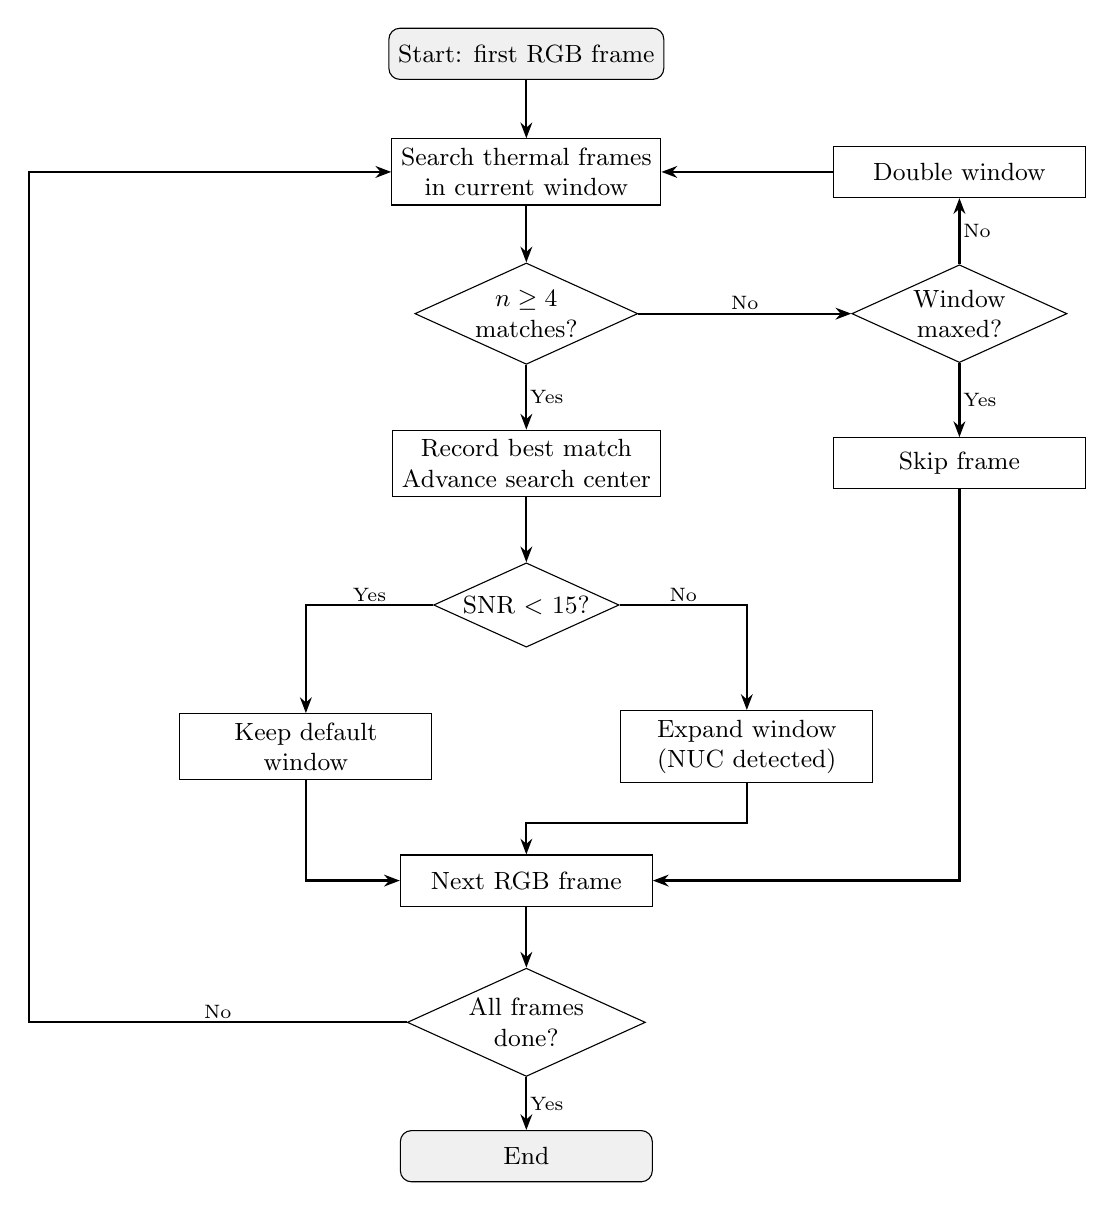
\begin{tikzpicture}[
    % Styles
    startstop/.style={
        rectangle, rounded corners=4pt,
        minimum width=3.2cm, minimum height=0.65cm,
        draw=black, fill=gray!12,
        font=\small, align=center
    },
    process/.style={
        rectangle,
        minimum width=3.2cm, minimum height=0.65cm,
        draw=black, fill=white,
        font=\small, align=center
    },
    decision/.style={
        diamond, aspect=2.2,
        draw=black, fill=white,
        font=\small, align=center,
        inner sep=1pt
    },
    arrow/.style={-{Stealth[length=2mm]}, thick},
    lbl/.style={font=\scriptsize, fill=white, inner sep=1pt}
]

% === COLUMN 1 (Main flow - center) ===
\node (init) [startstop] at (0, 0) {Start: first RGB frame};
\node (search) [process] at (0, -1.5) {Search thermal frames\\in current window};
\node (found) [decision] at (0, -3.3) {$n \geq 4$\\matches?};
\node (record) [process] at (0, -5.2) {Record best match\\Advance search center};
\node (quality) [decision] at (0, -7) {SNR $<$ 15?};

% === COLUMN 2 (Quality branches - spread left/right) ===
\node (reset) [process] at (-2.8, -8.8) {Keep default\\window};
\node (expand) [process] at (2.8, -8.8) {Expand window\\(NUC detected)};

% === COLUMN 3 (Retry loop - far right) ===
\node (maxwin) [decision] at (5.5, -3.3) {Window\\maxed?};
\node (double) [process] at (5.5, -1.5) {Double window};
\node (skip) [process] at (5.5, -5.2) {Skip frame};

% === BOTTOM (Loop control) ===
\node (next) [process] at (0, -10.5) {Next RGB frame};
\node (done) [decision] at (0, -12.3) {All frames\\done?};
\node (stop) [startstop] at (0, -14) {End};

% === ARROWS ===
% Main vertical flow
\draw [arrow] (init) -- (search);
\draw [arrow] (search) -- (found);

% Found match? -> Yes -> Record
\draw [arrow] (found) -- node[lbl, right] {Yes} (record);
\draw [arrow] (record) -- (quality);

% Quality branches
\draw [arrow] (quality) -| node[lbl, pos=0.25, above] {Yes} (reset);
\draw [arrow] (quality) -| node[lbl, pos=0.25, above] {No} (expand);

% Reset/Expand/Skip -> Next (from left, top, right)
\draw [arrow] (reset.south) |- (next.west);
\draw [arrow] (expand.south) -- ++(0, -0.5) -| (next.north);

% Found match? -> No -> Retry path
\draw [arrow] (found) -- node[lbl, above] {No} (maxwin);
\draw [arrow] (maxwin) -- node[lbl, right] {No} (double);
\draw [arrow] (double) -- (search);
\draw [arrow] (maxwin) -- node[lbl, right] {Yes} (skip);
% Skip enters from right (perpendicular)
\draw [arrow] (skip.south) |- (next.east);

% Main loop
\draw [arrow] (next) -- (done);
\draw [arrow] (done) -- node[lbl, right] {Yes} (stop);
% Route loop-back arrow far left to avoid "Keep default window" box
\draw [arrow] (done.west) -- node[lbl, above] {No} ++(-4.8, 0) |- (search.west);

\end{tikzpicture}

\caption{Temporal frame matching algorithm. For each RGB frame $i$, the algorithm searches thermal frames within a sliding window $[c_i - L, c_i + L]$ centered at the previous match. SuperPoint-SuperGlue detects and matches keypoints across modalities; the optimal thermal frame $j^*$ minimizes average Euclidean displacement $\bar{d}(i,j)$ between matched feature positions---since frames are spatially aligned, temporally coincident frames exhibit co-located features. Matching requires $n \geq 4$ correspondences after confidence filtering (top 50\% by descriptor distance); fewer matches trigger window expansion up to 200 frames. Quality metrics (SNR, gradient) detect NUC events and preemptively expand the next frame's window.}
\label{fig:temporal_flowchart}
\end{figure}



\subsection{Object Detection and Tracking}\label{subsec:detection_tracking}

We employ Detectron2~\citep{wu2019detectron2} with Mask R-CNN~\citep{he2017mask} fine-tuned on ThermalRGBTrash (Section~\ref{subsec:dataset}) for instance segmentation in the RGB domain. Raw predictions are refined via two-stage NMS:
\begin{equation}
\mathcal{P}_{\text{final}} = \mathbb{F}_{\text{NMS}}(\mathcal{P}, \tau_{\text{per-class}}, \tau_{\text{cross-class}})
\label{eqn:nms_overall}
\end{equation}
Per-class NMS (threshold $\tau_{\text{per-class}}$) eliminates redundant same-class detections; cross-class NMS (threshold $\tau_{\text{cross-class}}$) resolves inter-class ambiguity by retaining only the highest-confidence prediction when different classes overlap, ensuring each spatial region receives exactly one class label. Refined masks are transformed to the thermal domain via the homography $\mathbf{H}$. To associate per-frame masks into trajectories $\mathcal{T} = \{T_1, \ldots, T_M\}$ for thermal time-series extraction, we employ OC-SORT~\citep{cao2023ocsort}. This tracker suits conveyor applications where objects move at near-constant velocities; its observation-centric momentum computes velocity from recent detections rather than Kalman predictions alone, preventing drift during brief occlusions. OC-SORT parameters were optimized iteratively using three quality metrics: track continuity (proportion of tracks exceeding 100 frames), class consistency (agreement between per-frame predictions and track majority class), and fragmentation ratio. After five iterations, optimization converged to track continuity exceeding 85\% and mean class consistency above 96\%, confirming reliable trajectory extraction for downstream thermal analysis. Figure~\ref{fig:tracking_visualization} illustrates this cross-modal correspondence, showing instance segmentation masks in the RGB domain and their spatial alignment in the thermal frame after homography transformation.

\begin{figure}[t]
    \centering
    \begin{subfigure}[b]{0.48\textwidth}
        \centering
        \includegraphics[width=\textwidth]{images/tracked_rgb_frame.png}
        \caption{RGB frame with instance segmentation}
        \label{fig:tracked_rgb}
    \end{subfigure}
    \hfill
    \begin{subfigure}[b]{0.48\textwidth}
        \centering
        \includegraphics[width=\textwidth]{images/tracked_thermal_frame.png}
        \caption{Corresponding thermal frame}
        \label{fig:tracked_thermal}
    \end{subfigure}
    \caption{Cross-modal object tracking visualization. (a) RGB frame showing Mask R-CNN instance segmentation with OC-SORT track identifiers (131, 127, 137, 124). Colored overlays indicate per-instance masks from which class probability distributions are extracted. (b) Spatially aligned thermal frame (grayscale) after homography transformation, where identical track IDs enable thermal intensity measurement within warped mask boundaries. The thermal signatures reveal material-specific heat retention: plastic bottles (tracks 127, 131) exhibit elevated intensity compared to metal cans at frame edges.}
    \label{fig:tracking_visualization}
\end{figure}

\subsection{Object Classification}
This study evaluates object classification using both RGB and thermal domains independently. In the RGB domain, the segmentation network (Section~\ref{subsec:detection_tracking}) provides per-frame class predictions with associated probability distributions, which are aggregated across the object's track to derive an RGB-domain classification. In the thermal domain, classification is performed on the thermal intensity time-series within each object's tracked mask, capturing material-specific thermal signatures.

\subsubsection{RGB Domain Classification}\label{sec:rgb_classification}
To assess the class-discriminative potential of RGB-based predictions, we analyze the full four-class probability distribution from each frame. Rather than relying on scalar confidence values, we examine how probability mass distributes across all classes, revealing both model certainty and systematic confusion patterns.

Statistical analysis on training set of 330 tracked objects across four material classes reveals class-dependent recognition difficulty (Table~\ref{tab:spatial_class_summary}). Using the mean probability assigned to the correct class as our primary metric, glass achieves the highest correct probability, followed by metal, plastic, and paper. We define a separability index as the ratio of correct-class probability to the maximum wrong-class probability. Values above 50 indicate easy classification, while values below 25 indicate difficulty. Glass is the easiest one to discriminate, while metal and plastic require moderate discrimination effort; paper presents the greatest classification challenge.

\begin{table}[h]
\centering
\small
\caption{Per-class classification metrics from probability distributions.}
\label{tab:spatial_class_summary}
\begin{tabular}{lcccc}
\hline
Class & N & $P_{correct}$ & Primary Confuser & Separability \\
\hline
Glass & 89 & 91.1\% & Plastic (3.1\%) & 109.2 \\
Metal & 60 & 82.6\% & Plastic (5.9\%) & 47.5 \\
Plastic & 118 & 69.4\% & Paper (11.1\%) & 25.6 \\
Paper & 49 & 60.5\% & Plastic (20.2\%) & 22.2 \\
\hline
\end{tabular}
\end{table}

\begin{figure}[h]
    \centering
    \includegraphics[width=0.7\textwidth]{images/spatial_prob_confusion_heatmap.png}
    \caption{Mean probability distribution by ground truth class, revealing systematic model confusion patterns. The segmentation model assigns high probability to the correct class for glass (91.1\%) and metal (82.6\%), but exhibits substantial paper-plastic bidirectional confusion: paper objects leak 22.6\% probability to plastic, while plastic objects leak 14.2\% to paper.}
    \label{fig:spatial_confusion}
\end{figure}

The probability confusion matrix in Figure~\ref{fig:spatial_confusion} reveals systematic failure modes. The critical confusion pair is paper$\leftrightarrow$plastic, with bidirectional probability leakage (22.6\% paper$\rightarrow$plastic, 14.2\% plastic$\rightarrow$paper). This confusion in the RGB domain motivates exploration of thermal signatures, where paper and plastic may exhibit distinct thermal responses that resolve this ambiguity.

\subsubsection{Thermal Domain Classification}\label{sec:thermal_classification}
To assess the class-discriminative potential of thermal signatures, we extract five features from each object's thermal time-series: mean intensity ($\mu_I$), median intensity ($\tilde{I}$), standard deviation ($\sigma_I$), rise time ($t_r$), and fall time ($t_f$). These features capture complementary aspects of thermal behavior that differ systematically across material classes.

The temporal features capture heating and cooling dynamics: \textit{rise time} ($t_r$) measures frames to reach 70\% of peak intensity, while \textit{fall time} ($t_f$) measures frames from peak until cooling below 70\%. Table~\ref{tab:thermal_class_summary} presents per-class thermal statistics for the 330 training tracks. Glass occupies the low end of the intensity spectrum ($\mu_I = 61.8$) with minimal variability ($\sigma_I = 12.6$). Plastic exhibits the highest intensity ($\mu_I = 100.1$) and longest heat retention ($t_f = 631$ frames). Paper shows the highest thermal variability ($\sigma_I = 39.9$). Metal falls in the intermediate range ($\mu_I = 86.1$) with high variability ($\sigma_I = 31.2$), causing feature space overlap with adjacent classes.

\begin{table}[h]
\centering
\small
\caption{Per-class thermal feature statistics (mean $\pm$ std across tracks).}
\label{tab:thermal_class_summary}
\begin{tabular}{lccccc}
\hline
Class & $\mu_I$ & $\tilde{I}$ & $\sigma_I$ & $t_r$ (frames) & $t_f$ (frames) \\
\hline
Glass & 61.8 $\pm$ 13.4 & 64.0 $\pm$ 13.6 & 12.6 $\pm$ 4.2 & 766 $\pm$ 552 & 201 $\pm$ 357 \\
Metal & 86.1 $\pm$ 20.9 & 78.6 $\pm$ 18.3 & 31.2 $\pm$ 18.2 & 729 $\pm$ 559 & 368 $\pm$ 242 \\
Plastic & 100.1 $\pm$ 23.0 & 97.0 $\pm$ 22.3 & 32.1 $\pm$ 12.6 & 487 $\pm$ 182 & 631 $\pm$ 259 \\
Paper & 95.0 $\pm$ 25.9 & 86.5 $\pm$ 29.7 & 39.9 $\pm$ 14.7 & 496 $\pm$ 213 & 359 $\pm$ 150 \\
\hline
\end{tabular}
\end{table}

\begin{figure}[h]
    \centering
    \begin{subfigure}[b]{0.48\textwidth}
        \centering
        \includegraphics[width=\textwidth]{images/thermal_feature_3d_plot_mean_vs_median_vs_stddev.png}
        \caption{Intensity features: glass clusters at low values; plastic occupies the high-intensity region.}
        \label{fig:mean_vs_median}
    \end{subfigure}
    \hfill
    \begin{subfigure}[b]{0.48\textwidth}
        \centering
        \includegraphics[width=\textwidth]{images/thermal_feature_3d_plot_stddev_vs_timedynamics.png}
        \caption{Temporal dynamics: plastic shows longest fall times; metal-paper separable via variability.}
        \label{fig:stddev_vs_dynamics}
    \end{subfigure}
    \caption{3D scatter plots of 330 training tracks demonstrating class separability in the thermal feature space. The four material classes occupy geometrically distinct regions, confirming feasibility of thermal-based classification.}
    \label{fig:thermal_features}
\end{figure}

The thermal feature space exhibits class-dependent separability, as shown in Figure~\ref{fig:thermal_features}. Glass and plastic occupy opposite ends of the intensity spectrum with a 38-unit gap ($\mu_I = 61.8$ vs.\ $100.1$), enabling clear discrimination. Metal ($\mu_I = 86.1$) and paper ($\mu_I = 95.0$) occupy intermediate positions with substantial overlap, consistent with these classes being the most challenging to classify. Additional separation is provided by temporal dynamics: plastic shows the longest fall time ($t_f = 631$ frames), while glass cools most rapidly ($t_f = 201$ frames).

\subsubsection{Experimental Protocol}\label{subsec:protocol}

To ensure methodologically rigorous comparison, all deep learning classifiers share identical experimental conditions: (i) the stratified train, validation, test split defined in Table~\ref{tab:dataset_combined} with fixed random seed (42), (ii) Bayesian hyperparameter optimization via Optuna (20 trials, 5-fold cross-validation), (iii) unified training procedures (AdamW optimizer, ReduceLROnPlateau scheduler, early stopping with patience 15), (iv) consistent time-series augmentation (time masking, magnitude scaling, time warping, cutout), and (v) class-weighted cross-entropy loss to address label imbalance.

\section{Results and Discussion}

\subsection{Image Registration Evaluation}

Registration accuracy was evaluated comprehensively across all 19 experiments, analyzing 281,439 matched frame pairs to ensure statistically robust error estimation. Spatial registration quality is measured by mean reprojection error computed on inlier correspondences:
\begin{equation}\label{eqn:RE_spatial_l2}
    RE_{\text{spatial}} = \frac{1}{M} \sum_{i=1}^{M} \|\tilde{p}_i - \hat{p}_i\|_2
\end{equation}
where $M$ is the number of inlier matches (RANSAC threshold 10\,px), $\tilde{p}_i$ are detected SuperPoint feature positions in the thermal image, and $\hat{p}_i = H p_i$ are the corresponding warped positions from the RGB image. Temporal registration error aggregates feature displacement across all $N_w$ frame matches:
\begin{equation}
    RE_{\text{temporal}} = \sum_{i=1}^{N_w} \bar{d}(i, j^*_i)
    \label{eqn:temporal_error}
\end{equation}
where $j^*_i$ is the optimal matching thermal frame for RGB frame $i$ (Equation~\ref{eqn:optimal_frame}), and $\bar{d}(i, j^*_i)$ is the mean Euclidean distance between matched SuperPoint-SuperGlue keypoints in that frame pair. For each RGB frame, SuperPoint extracts keypoints in both the warped RGB frame and all candidate thermal frames within the search window; SuperGlue matches corresponding keypoints across modalities. The mean displacement $\bar{d}$ quantifies alignment quality for each matched pair, with lower values indicating better spatial correspondence at the selected temporal offset. We report Mean Temporal Registration Error (MTRE = $RE_{\text{temporal}}/N_w$), Jitter Coefficient quantifying frame-to-frame stability:
\begin{equation}
    JC = \frac{\sigma_{\Delta j}}{\mu_{|\Delta j|}}
    \label{eqn:jitter_coeff}
\end{equation}
where $\Delta j = j^*_i - j^*_{i-1}$ represents consecutive matched frame differences, Monotonicity Score (MS = fraction of frames where $\Delta j > 0$), and Coverage (fraction of successfully matched frames). Table~\ref{tab:registration_metrics} summarizes performance metrics computed across all experiments.

\begin{table}[h]
\centering
\caption{Registration performance across 19 experiments (281,439 matched frame pairs). Spatial metrics computed per-experiment; temporal metrics aggregated across all frames.}
\label{tab:registration_metrics}
\begin{tabular}{@{}llcccc@{}}
\toprule
\textbf{Domain} & \textbf{Metric} & \textbf{Mean} & \textbf{Std} & \textbf{Median} & \textbf{Range} \\
\midrule
\multirow{3}{*}{Spatial} & Reprojection Error (px) & 2.27 & 0.48 & 2.19 & [1.67, 3.64] \\
& Inlier Rate (\%) & 99.1 & 0.8 & 99.3 & [97.2, 99.9] \\
& Inlier Count & 143 & 38 & 137 & [89, 241] \\
\midrule
\multirow{4}{*}{Temporal} & MTRE (px) & 4.68 & 1.55 & 3.99 & [2.87, 8.85] \\
& Jitter Coefficient & 1.87 & 0.34 & 1.79 & [1.35, 2.40] \\
& Monotonicity Score & 0.458 & 0.08 & 0.46 & [0.31, 0.58] \\
& Coverage & 0.9997 & 0.0004 & 0.9999 & [0.998, 1.0] \\
\bottomrule
\end{tabular}
\end{table}

Spatial registration achieved mean reprojection error of $2.27 \pm 0.48$ pixels (Equation~\ref{eqn:RE_spatial_l2}), with sub-3-pixel accuracy despite the cross-spectral modality gap between RGB and thermal imagery. The 99.1\% inlier rate confirms RANSAC successfully rejected outlier correspondences arising from cross-modal matching artifacts. At thermal resolution, this 2.27\,px error corresponds to 0.71\% of image width.

Temporal registration achieved MTRE of $4.68 \pm 1.55$\,px across 281,439 frame pairs (Equation~\ref{eqn:temporal_error}), with per-experiment values ranging from 2.87\,px (best) to 8.85\,px (worst). Near-perfect coverage (99.97\%) indicates successful correspondence for virtually all frames. The Jitter Coefficient of $1.87 \pm 0.34$ (Equation~\ref{eqn:jitter_coeff}) quantifies temporal stability: a JC of 1.87 indicates that the standard deviation of consecutive frame differences equals 1.87 times their mean absolute value, reflecting moderate variability in frame-to-frame matching. The moderate Monotonicity Score (0.458) arises from NUC compensation: when Non-Uniformity Correction events cause the thermal camera to pause, the algorithm permits backward temporal jumps to maintain spatial correspondence.

The total registration error (Equation~\ref{eqn:total_RE}) decomposes into spatial (32.7\%) and temporal (67.3\%) components, as visualized in Figure~\ref{fig:error_decomposition}. This reveals that temporal synchronization, rather than geometric transformation, constitutes the dominant error source, with practical implications: improvements to temporal synchronization (e.g., hardware triggering) would yield greater accuracy gains than further spatial refinement.

\begin{figure}[h]
\centering
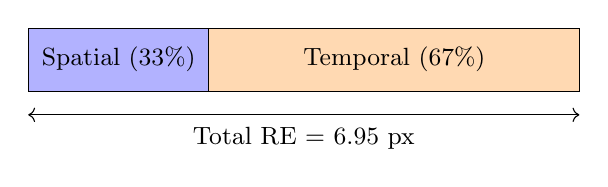
\begin{tikzpicture}
\draw[fill=blue!30] (0,0) rectangle (2.29,0.8);
\draw[fill=orange!30] (2.29,0) rectangle (7,0.8);
\node at (1.15,0.4) {\small Spatial (33\%)};
\node at (4.65,0.4) {\small Temporal (67\%)};
\draw[<->] (0,-0.3) -- (7,-0.3);
\node at (3.5,-0.6) {\small Total RE = 6.95 px};
\end{tikzpicture}
\caption{Decomposition of total registration error into spatial (2.27\,px) and temporal (4.68\,px) components.}
\label{fig:error_decomposition}
\end{figure}

\subsection{Thermal Classification Results}
\label{sec:thermal_results}

We evaluate eight classification methods on 110 test tracks using thermal intensity time-series (Table~\ref{tab:thermal_classifier_comparison}). All deep learning methods used identical training protocols (Section~\ref{subsec:protocol}) to ensure fair comparison.

SVM with five statistical features achieves the highest F1 macro (0.678), closely followed by BiGRU (0.676) and InceptionTime (0.672). The competitive performance of SVM suggests that summary statistics (mean, median, standard deviation, rise time, fall time) capture much of the discriminative information in thermal time-series, though deep learning methods achieve complementary strengths: BiGRU obtains the highest per-class F1 for glass (0.815), metal (0.636), and plastic (0.716), while SVM excels on paper (0.732). MiniRocket (0.644) and BiLSTM (0.614) achieve moderate performance. TCN (0.484), CNN-1D (0.491), and Transformer (0.324) underperform, with Transformer failing to learn meaningful thermal patterns.

\begin{table}[htbp]
\centering
\caption{Thermal classification performance comparison (n=110 test tracks). Best values in bold. F1 scores are macro-averaged; per-class columns show F1 scores.}
\label{tab:thermal_classifier_comparison}
\begin{tabular}{@{}lcccccc@{}}
\toprule
\textbf{Method} & \textbf{Accuracy} & \textbf{F1 Macro} & \textbf{Glass} & \textbf{Metal} & \textbf{Paper} & \textbf{Plastic} \\
\midrule
SVM (5 features) & 68.2 & \textbf{0.678} & 0.786 & 0.490 & \textbf{0.732} & 0.703 \\
BiGRU & \textbf{69.1} & 0.676 & \textbf{0.815} & \textbf{0.636} & 0.537 & \textbf{0.716} \\
InceptionTime & 68.2 & 0.672 & 0.764 & 0.609 & 0.615 & 0.700 \\
MiniRocket & 65.5 & 0.644 & 0.754 & 0.553 & 0.611 & 0.658 \\
BiLSTM & 63.6 & 0.614 & 0.688 & 0.526 & 0.550 & 0.692 \\
CNN-1D & 50.9 & 0.491 & 0.778 & 0.286 & 0.386 & 0.514 \\
TCN & 54.5 & 0.484 & 0.565 & 0.286 & 0.424 & 0.660 \\
Transformer & 32.7 & 0.324 & 0.400 & 0.217 & 0.393 & 0.286 \\
\midrule
\multicolumn{7}{l}{\textit{Baseline}} \\
Gundupalli$^{a}$ & 55.5 & 0.550 & 0.760 & 0.370 & 0.540 & 0.530 \\
\bottomrule
\end{tabular}
\vspace{1mm}

\footnotesize{$^{a}$Peak thermal features (mean + std around peak frame)~\citep{GUNDUPALLI201713}.}
\end{table}

Per-class analysis reveals material-specific classification difficulty. Glass is most reliably classified (best F1 = 0.815 by BiGRU), consistent with its distinctively low thermal intensity ($\mu_I = 61.8$) that separates it from all other classes. Plastic achieves the second-highest F1 (0.716 by BiGRU), reflecting its characteristic high thermal intensity ($\mu_I = 100.1$) and long heat retention ($t_f = 631$ frames). Metal is the most challenging class (best F1 = 0.636 by BiGRU), due to its high thermal variability ($\sigma_I = 31.2$) causing overlap with both paper and plastic in the feature space. Paper shows variable results across methods (F1 ranging from 0.386 to 0.732), with SVM capturing paper's intermediate thermal profile most effectively.

To quantify the contribution of temporal dynamics beyond peak statistics, we implemented the peak histogram classifier of \citet{GUNDUPALLI201713}, which extracts peak intensity and $\pm$50-frame standard deviation. This baseline achieves F1 = 0.550, and the 0.128 pp gap versus SVM demonstrates that richer feature representations, including rise/fall time dynamics, provide additional material-discriminative information beyond peak statistics alone.


\section{Conclusion}

This paper presented a thermal imaging framework for conveyor-based waste classification. The contributions are: (1) a spatial-temporal registration method achieving 2.27-pixel spatial and 4.68-pixel temporal alignment across 281,439 frame pairs without hardware synchronization; (2) a systematic benchmark of eight thermal classification methods on 550 tracked object trajectories, with SVM (F1 = 0.678) and BiGRU (F1 = 0.676) achieving the best performance; (3) evidence that sequence-based classification (SVM F1 = 0.678) outperforms peak histogram features (Gundupalli F1 = 0.550), confirming that temporal shape encodes material-discriminative information; and (4) release of ThermalRGBTrash, an RGB-thermal dataset of 550 registered object trajectories. The moderate classification performance (best F1 = 0.678) indicates that thermal signatures alone provide partial material discrimination, with glass most reliably classified (F1 = 0.786) and metal most challenging (F1 = 0.490).

\bibliographystyle{elsarticle-harv}
\bibliography{references} % Assumes a references.bib file

\end{document}
